\documentclass[noindent]{tudreport}
\usepackage[utf8]{inputenc}
\usepackage[german]{babel}
\usepackage{amsmath}
\usepackage{listings}
\title{TUDas - Organisationsapp der Technischen Universität Darmstadt}
\subtitle{Ergebnis des E-Learning Projektpraktikums WS18-19}
\subsubtitle{Benedikt Lins (1799381) und Stefan Thaut (1800351)\\
			Fachbereich 20 - Informatik\\
			\today}
\setlength{\parindent}{0em} 

\DeclareMathOperator{\start}{start}
\DeclareMathOperator{\getEnd}{end}
\DeclareMathOperator{\hour}{hour}

\begin{document}
	\lstset{language=Java}
	\maketitle
	\tableofcontents
	
	\chapter{Motivation}
		Jeder Student oder der, der einmal einer gewesen ist, kennt es: Du kommst das erste Mal in die Uni und hast keine Ahnung, was zu tun ist. Alles ist komplett neu und Du bist froh, wenn Du die Räume findest, in denen Du Dich laut Deinem Willkommensbrief einfinden sollst. Selbst wenn Du dann nach ein paar Tagen herausgefunden hast, welche Straßenbahn Dich in die Uni bringt, bist Du nach ein paar Wochen immer noch ratlos, welche Dokumente du gegebenenfalls wo nachreichen musst, wo Du Dich zu welchen Veranstaltungen und Prüfungen anmelden sollst und in welchem Kellerraum nun dieser Treffpunkt Mathe stattfindet.\\
		
		Diesem Problem soll sich die (Android-)App \textit{TUDas} widmen. Die App soll als Organisationsplattform für Studenten verschiedener Fachbereiche während ihres ersten Semesters dienen. Dabei soll TUDas vorhandene Plattformen, wie \textit{Moodle}\footnote{www.moodle.tu-darmstadt.de [zuletzt aufgerufen: 23.11.2018]} oder die \textit{OAPP} \footnote{www.oapp.tu-darmstadt.de [zuletzt aufgerufen: 23.11.2018]} unterstützen und nicht ersetzen.\\
		%TODO worin unterscheidet sich die App von OAPP und Moodle und Google Maps etc?
		
		Diese Dokumentation soll einerseits die Funktionalitäten der App TUDas festhalten und andererseits als Übersicht für zukünftige Entwickler dienen. Kapitel \ref{chap:technical_specifications} behandelt die technischen Spezifikationen der App. In Kapitel \ref{chap:functionalities} werden die Features beschrieben, die von der App in ihrer jeweils aktuellen Version angeboten werden. Und Kapitel \ref{chap:documentation} beinhaltet eine Dokumentation des Codes.
		
	\chapter{Einrichtung}\label{chap:setup}
		Für das Funktionieren der App muss auf Seiten der Entwickler, abgesehen von der Verbreitung der App, lediglich ein Webserver mit zwei Frameworks aufgesetzt werden. Für das Webinterface \textit{Edidas} wird das Framework cakePHP\footnote{https://book.cakephp.org/3.0/en/installation.html [zuletzt aufgerufen: 28.03.2019]} in der Version 3.7 verwendet. Die REST-API wird über das Slim-Framework\footnote{http://www.slimframework.com/docs/v3/start/installation.html [zuletzt aufgerufen: 28.03.2019]} realisiert. Ist der Webserver entsprechend der in den Fußnoten genannten Anleitungen eingerichtet, so muss lediglich der gelieferte Code auf den Webserver kopiert werden.
	
	\chapter{Funktionalitäten}\label{chap:functionalities}
		Dieses Kapitel beschreibt die Funktionalitäten, die die App in ihrer jeweils aktuellen Version anbietet. Dabei sollen die jeweiligen funktionalen sowie nicht-funktionalen Anforderungen aufgezeigt werden und nicht die programmiertechnische Umsetzung, die dann in Kapitel \ref{chap:documentation} folgt.
		
		\section{Campus-Navigation}\label{sec:campus_navigation}
			Die TU Darmstadt belegt Gebäude und Räume, die über das gesamte Stadtgebiet verteilt sind. Daher kann es schwer fallen, stets zu wissen, wohin man gehen muss, um pünktlich zu dem Raum zu gelangen, in dem die nächste Veranstaltung stattfindet. Der Nutzer soll deswegen die Möglichkeit haben, zu dem entsprechenden Ort einer Veranstaltung navigieren zu können.
		
		\section{Stundenplan}\label{sec:timetable}
			Im Stundenplan werden die selbst erstellten Termine des Nutzers angezeigt. Hier können grundsätzlich zwei Typen von Terminen unterschieden werden:
			\begin{itemize}
				\item Einfache Termine
				
				\item Wiederholende Termine
			\end{itemize}
			Die Charakteristik der einfachen Termine impliziert eine einmalige Anzeige im Stundenplan an einem bestimmten Datum. Daher ist es sinnvoll, den Stundenplan datumsabhängig anzuzeigen. Da die Bildschirmbreite des Smartphones in der vertikalen Ausrichtung deutlich begrenzt ist, muss auch die Anzahl der angezeigten Tage beschränkt werden. Diese Beschränkung kann der Nutzer selbst vornehmen und zwischen zwei und fünf anzuzeigenden Tagen wählen. Weniger als zwei Tage ist nicht sinnvoll, da sich dies mit der Funktionalität überschneiden würde, die in \ref{sec:todo_list} beschrieben ist. Bei mehr als fünf anzuzeigenden Tagen ist die Grenze der visuellen Darstellbarkeit schnell erreicht. Darüber hinaus besteht eine Werktagswoche in der Regel aus fünf Tagen. Der ausgewählte Zeitraum wird in einer Kopfzeile über den Tageslisten angezeigt. Auf der linken Seite sind in vertikaler Ausrichtung die Uhrzeiten in stündlichem Abstand untereinander angeordnet. Dabei beginnt der Stundenplan oben mit der maximalen ganzen Stunde, die kleiner als oder gleich allen Anfangsuhrzeiten von Terminen im angezeigten Zeitraum ist und endet unten mit der minimalen ganzen Stunde, die größer als oder gleich allen Enduhrzeiten der gleichen Termine sind.
		
		\section{Variabel einsetzbare, moderierbare Aufgabenlisten}\label{sec:todo_list}
			Da Erstsemesterstudenten oft nicht wissen, welche Termine und Veranstaltung für sie wichtig sind, ist es sinnvoll, diese Termine bereitzustellen. Dies setzt voraus, dass solche Termine von einer externen Institution erstellt und editiert werden. Eine solche Funktionalität benötigt einen zentralen Speicherort, wo die erstellten Termine gespeichert und von der App abgerufen werden können.\\
			Auf der anderen Seite gibt es spezifische Termine, die nicht jeder Student angezeigt bekommen soll, um nicht mit Informationen überflutet zu werden. Hierfür soll eine Art Abonnement-System etabliert werden, mittels dem Studenten verschiedene Labels abonnieren können, unter denen Informationen zu dem gleichen Thema zusammengefasst werden. Diese Labels können vollkommen frei gewählt werden und können beispielsweise für verschiedene Lehrveranstaltungen (z.B. eine Vorlesung) aber auch für die Termine der Orientierungsphase stehen.\\
			Um solche Termine zu erstellen und zu bearbeiten, wird ein Webinterface mit einer zugrundeliegenden Datenbank verwendet, welches über einen herkömmlichen Browser erreichbar ist. Fachschaften und andere Institutionen benutzen oftmals schon eine Software für die Verwaltung ihrer Termine. Daher soll das Webinterface auch eine Importfunktion besitzen, die das Hochladen von Kalenderdateien ermöglicht und für verschiedene Dateiformate erweiterbar ist.\\\\
			Die Termine von abonnierten Terminlisten werden dem Nutzer in einer Tagesansicht des jeweils aktuellen Tags angezeigt, welche gleichzeitig auch die Startseite der App darstellt. Zusätzlich enthält diese Ansicht ebenfalls alle privaten Termine, die der Nutzer im Stundenplan erstellt hat. Die Termine werden hier unabhängig von ihrer Länge in gleich großen Blöcken angezeigt und nach ihrem Startzeitpunkt sortiert.\\
			Viele Nutzer verwenden üblicherweise eine andere Applikation zur Verwaltung ihres Kalenders. Daher werden für alle angezeigten Termine in der Tagesansicht überprüft, ob sich diese mit einem Termin einer anderen installierten Kalenderapp überschneidet. Ist dies der Fall, wird dies in dem Block des Termins durch ein Icon angezeigt.
		
	\chapter{Dokumentation der Implementierung}\label{chap:documentation}
		\section{Campus-Navigation}
			Um die in Abschnitt \ref{sec:campus_navigation} beschriebene Funktionalität erfüllen zu können, kann für einen Termin ein Ort gespeichert werden. Dabei ist es dem Nutzer selbst überlassen, was er hierbei eingibt. Für die Realisierung der Navigation haben sich verschiedene Möglichkeiten geboten:
			\begin{itemize}
			\item Nutzen einer Karten-API, um sowohl den kürzesten Weg zu finden als auch den Weg auf einer Karte anzuzeigen
			
			\item Crawlen von Kartenmaterial und der Entwurf eines eigenen Routing-Algorithmus
			
			\item Weiterleitung an eine Navigationsapp
			\end{itemize}
			
			Die meisten APIs, die einen Navigationsalgorithmus bereitstellen, sind entweder kostenpflichtig oder begrenzen die Anzahl der Zugriffe für einen bestimmten Zeitraum auf ein Maß, das für den erwarteten Nutzungsumfang von TUDas unzureichend ist. Aus Gründen der Kosteneffizienz der App ist die Nutzung einer Karten-API daher nicht möglich.\\
			Eine weitere Möglichkeit, die Campus-Navigation zu realisieren, ist das Crawlen, also das Beschaffen von frei zugänglichem Kartenmaterial wie zum Beispiel von Openstreetmap. %TODO Link einfügen
			Hier wird Kartenmaterial in einem verarbeitungsfähigen Format bereitgestellt. Auf dieser Grundlage kann dann ein Algorithmus wie etwa der Dijkstra entwickelt, bzw. angewandt werden, um eine kürzeste Route von der aktuellen Position des Nutzers bis zum angegebenen Ziel zu berechnen. Auch dieser Ansatz muss aus verschiedenen Gründen abgelehnt werden. Einerseits enthalten die verfügbaren Kartendaten sehr viele Informationen, die für die Anwendung der App unnötig sind, weshalb ein hoher Aufwand aufgebracht werden muss, um die Daten zu bereinigen. Darüber hinaus müssten die Daten ständig aktualisiert werden, um mögliche Straßensperrungen oder Änderungen des Kartenmaterials einbinden zu können. Andererseits muss die Korrektheit des Routing-Algorithmus gewährleistet werden, was im Umfang dieser Implementierung nicht möglich ist.\\
			Daher wird im Umfang dieses Projekts die Aufgabe der Navigation an eine externe App abgegeben. Hier bietet sich die Navigationsapp von Google "Google Maps" an. Diese App ist in der Regel auf allen Android Smartphones installiert oder verfügbar. Darüber hinaus stellt diese App eine API bereit, die Navigationsanfragen von anderen Apps begünstigt.
			
		\section{Stundenplan}\label{sec:impl_timetable}
			Wie in Abschnitt \ref{sec:timetable} beschrieben, müssen grundlegend zwei Arten von Terminen unterschieden werden. Um zukünftig auch wiederholende Termine unterstützen zu können, ist die Modellierung im Vorhinein dahingehend angepasst. Ein wiederholender Termin hat im Vergleich zu einem einfachen Termin zusätzlich ein Startdatum, an dem die Wiederholung des Termins beginnt und ein Enddatum, wann die Wiederholung endet. Notwendig ist ebenfalls eine Wiederholungsvorschrift. Möchte man nun eine Teilmenge von wiederholenden Terminen löschen, so ist es notwendig, dass die Termine nicht zur Laufzeit auf Grundlage der Wiederholungsvorschrift berechnet werden sondern die Termine schon gespeichert wurden. Ansonsten wäre es nicht möglich zu spezifizieren, welche Termine von der Wiederholungsvorschrift ausgeschlossen werden sollen. Die wiederholenden Termine unterscheiden sich dann nur noch in den Daten. Der Titel und die Beschreibung beispielsweise sind für alle wiederholenden Termine jeweils gleich. Um Redundanzen zu vermeiden, werden solche Attribute von den reinen Datumsangaben getrennt. Die Klasse \lstinline!AppointmentContent! beinhaltet die statischen Informationen einer Terminsammlung und die Klasse \lstinline!Appointment! enthält die Datumsangaben. Die Attribute der Klassen sind im UML-Diagramm in Abbildung \ref{fig:uml_appointment} zu sehen.\\
			Für eine mathematische Beschreibung des Projekts müssen diverse Hilfsfunktionen definiert werden. Sei $A$ die Menge aller Termine des Benutzers und $\mathbb{D}$ die Menge aller Datumsangaben, die auch den Zeitpunkt am Tag beinhalten. Die Funktion
			\begin{align}
\start: A \rightarrow \mathbb{D} \label{fun:start}
			\end{align}
			liefert für einen gegebenen Termin den Startzeitpunkt. Analog liefert die Funktion
			\begin{align}
\getEnd: A \rightarrow \mathbb{D} \label{fun:end}
			\end{align}
			den Endzeitpunkt des gegebenen Termins. Für eine bestimmte Datumsangabe gibt die Funktion
			\begin{align}
\hour: \mathbb{D} \rightarrow \{0, \dots, 23\} \label{fun:hour}
			\end{align}
			die Stunde der Angabe aus.
			
			\begin{figure}[h]
				\centering
				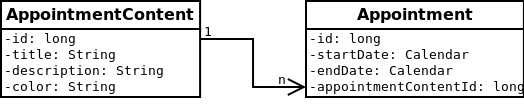
\includegraphics[scale=0.5]{img/uml_appointment.png}
				\caption{UML-Diagramm der Klassen \lstinline!AppointmentContent! und \lstinline!Appointment!}
				\label{fig:uml_appointment}
			\end{figure}
			
			\subsection{Modellierung der Anfangs- und Endzeitbedingung}
				Die in Abschnitt \ref{sec:timetable} beschriebene Anforderung, dass der Stundenplan mit der maximalen Stunde beginnen soll, die kleiner als die Startzeiten aller Termine im betrachteten Zeitraum ist, kann wie folgt formalisiert werden: Für ein gegebenes Start- und Enddatum $s \in \mathbb{D}$, bzw. $e \in \mathbb{D}$ ist
				\begin{align}
A_f = \{a \in A: s \leq a \leq e\}
				\end{align}
				die Menge aller Termine im gegebenen Zeitraum. Dann ist die gesuchte Stunde $h$, zu der der Stundenplan beginnen soll, mithilfe der Funktionen \ref{fun:start} und \ref{fun:hour} wie folgt definiert:
				\begin{align}
h_s = \max\{h_s \in \{0, \dots, 23\}: \forall a \in A_f: h_s \leq \hour(\start(a)) \}
				\end{align}
				Analog ist die Stunde der Endzeit $h_e$ definiert:
				\begin{align}
h_e = \min\{h_e \in \{0, \dots, 23\}: \forall a \in A_f: h_e \geq \hour(\getEnd(a)) \}
				\end{align}
			
			\subsection{Positionierung der Termine im Stundenplan}
				Die Termine sollen in einem tabellenartigen Format angezeigt werden. Dabei soll jede Spalte der Tabelle einen Tag repräsentieren. Innerhalb eines Tages sollen die Termine untereinander angezeigt werden. Programmtechnisch wird jeder Tag über ein Layout beschrieben, dem Elemente vertikal hinzugefügt werden können. Für Zeiten, zu denen kein Termin existiert, wird dem Layout ein leeres Feld hinzugefügt. Damit beschränkt sich die korrekte Positionierung der Termine auf das Berechnen der Höhen der einzelnen Elemente. Dazu wird eine Konstante $L$ eingeführt, die die Anzahl der Pixel pro Minute angibt. Die Dauer eines Termins wird dann in Minuten berechnet und mit der Konstante multipliziert, um die entsprechende Höhe zu berechnen.
	
	\chapter{Codespezifische Dokumentation}
		In diesem Kapitel soll ein konkreter Überblick über den Code gegeben werden.
		
		\section{Struktur}
			TUDas ist ein Android-Projekt und hält sich an das MVVM-Entwurfsmuster\footnote{https://developer.android.com/jetpack/docs/guide [zuletzt aufgerufen: 28.03.2019]}. Die Klassen in der Projektstruktur sind nach ihren Aufgaben in Packages unterteilt. Es existieren die folgenden Packages:
			\begin{itemize}
			\item adapters: Adapter zur Darstellung von Listen mit variabler Größe
			
			\item customWidgets: Eigens erstellte Komponenten zur Anzeige innerhalb von Views
			
			\item fragments
			
			\item listeners: Listener, die in mehreren Klassen referenziert werden
			
			\item localdatabase: Klassen für die lokale Persistenz über eine Room-Datenbank
			
			\item model: Model-Klassen, die in der Datenbank gespeichert werden können
			
			\item repositories: Datenrepositories, die verschiedene Datenquellen zusammenfassen
			
			\item utils: Utility-Funktionen, die in mehreren Klassen referenziert werden
			
			\item viewmodels: Viewmodels für alle Activities
			
			\item views: Eigens erstellte Views, die in Activities genutzt werden
			\end{itemize}
			
			Das Projekt beinhaltet darüber hinaus fünf Activities:
			\begin{itemize}
			\item DailyApointmentsActivity: Tagesansicht der Termine, die aus der Room-Datenbank und der zentralen Datenbank auf dem Server geladen werden; Einstiegspunkt der App
			
			\item ManageLabelActivity: Verwalten der abonnierten Listen
			
			\item NewAppointmentActivity: Interface zum Hinzufügen eines neuen Termins in den Stundenplan
			
			\item SettingsActivity: Einstellungen der App
			
			\item TimeTableActivity: Darstellung eines Stundenplans mit mehreren Tagen
			\end{itemize}
			
			Die App ist für den Export auf andere Entwicklungsumgebungen wartungsarm gestaltet und muss kaum konfiguriert werden. Die URL der REST-API, über die die Termine in der zentralen Datenbank auf dem Server abgerufen werden, kann in der Klasse \textit{TudasServiceGenerator} im Package \textit{Model} gesetzt und verändert werden.
	
	\chapter{Ausblick}
		In diesem Kapitel sollen zuletzt noch Vorschläge unterbreitet werden, wie das Projekt weitergeführt werden kann. Diese Vorschläge haben es teilweise aus zeitlichen Gründen nicht in die aktuelle Version geschafft, da erst einmal die Grundfunktionalitäten erstellt werden mussten.
		
		\section{Erstellen von sich wiederholenden Terminen}
			Wie in Abschnitt \ref{sec:impl_timetable} beschrieben, wurde die Modellierung der Termine so gestaltet, dass sich Termine auch wiederholen können. Hier kann die Benutzerschnittstelle dahingehend angepasst werden, dass der Nutzer eine Wiederholungsvorschrift definieren kann und die Termine entsprechend dieser Vorschrift berechnet und mit dem Termininhalt assoziiert werden. Auch für die Weboberfläche von Edidas kann diese Funktionalität erstellt werden.
		
		\section{Wechseln des Starttages im Stundenplan durch Wischen}
			In der Stundenplanaktivität kann der angezeigte Zeitraum verändert werden, indem der Starttag über den Datepicker, der über die Datumszeile erreichbar ist, gewechselt wird. Ein erwartetes Verhalten im Stundenplan ist das Wechseln des Tages über eine horizontale Wischoperation. Hierfür muss das Layout der Stundenplanaktivität angepasst werden und ein eigener Gesture-Listener erstellt werden.
		
		\section{Tutorial}
			Sollte sich bei dem ersten Einsatz der App oder der Weboberfläche herausstellen, dass diese nicht selbst erklärend ist, sollte überlegt werden, eine Hilfe- oder Erklärungsfunktion in beide Systeme einzubauen. In dieser sollen dann die Funktionen der App oder der Weboberfläche erläutert werden.
			

\end{document}